\documentclass[12pt]{article}


\usepackage{amsmath, amssymb}

\usepackage{tikz}
\usetikzlibrary{graphs,quotes,arrows.meta}
\usetikzlibrary{automata,positioning}
\usetikzlibrary{shapes,arrows}
\usetikzlibrary{chains}
\usetikzlibrary{matrix,backgrounds}
\usetikzlibrary{calc}


\begin{document}


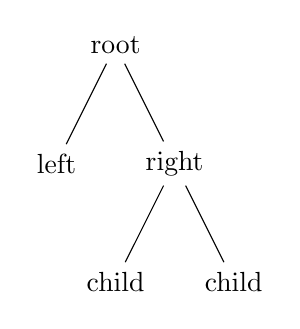
\begin{tikzpicture}
\node {root}
child {node {left}}
child {node {right}
	child {node {child}}
	child {node {child}}
};
\end{tikzpicture}



\vspace{50pt}




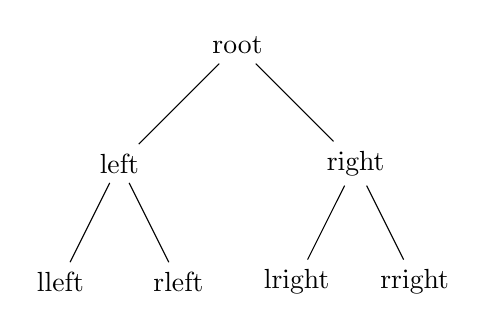
\begin{tikzpicture}[level distance=1.5cm,
  level 1/.style={sibling distance=3cm},
  level 2/.style={sibling distance=1.5cm}]
  \node {root}
    child {node {left}
      child {node {lleft}}
      child {node {rleft}}
    }
    child {node {right}
    child {node {lright}}
      child {node {rright}}
    };
\end{tikzpicture}



\vspace{50pt}



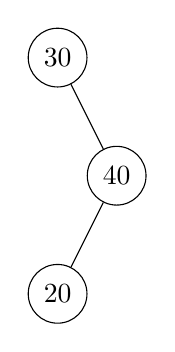
\begin{tikzpicture}
\node[circle,draw](z){$30$}
  child[missing]{}
  child{ node[circle,draw]{40} 
	  child{ node[circle,draw] {20} } 
	  child[missing] 
  };
\end{tikzpicture}





\vspace{50pt}






\begin{tikzpicture}
\node {$q_{1}$}
child {node {$q_{4}$}}
child {node {$q_{1}$}
	child {node {$q_{2}$}}
	child {node {$q_{1}$}
		child {node {$q_{1}$}
				child {node {$q_{1}$}}
				child {node {$q_{4}$}}
		}
		child {node {$q_{4}$}
			child {node {$q_{5}$}}
		}
	}
};
\end{tikzpicture}




\vspace{50pt}




\begin{tikzpicture}[sibling distance=3cm]
\node {$S$}
child {node {$a$}}
child {node {$b$}}
child {node {$S$}
	child {node {$a$}}
}
child {node {$b$}};
\end{tikzpicture}





\vspace{50pt}



\begin{tikzpicture}
\node {$S$}[sibling distance=3cm]
child {node {$a$}}
child {node {$A$}[sibling distance=2cm]
	child {node {$b$}}
	child {node {$S$}
		child {node {$a$}}
	}
}
child {node {$b$}};
\end{tikzpicture}




\vspace{50pt}




\begin{tikzpicture}
\node {$S$}[sibling distance=3cm]
child {node {$a$}}
child {node {$A$}[sibling distance=2cm]
	child {node {$S$}
		child {node {$a$}}
	}
	child {node {$b$}}
	child {node {$A$}
		child {node {$b$}}
		child {node {$a$}}
	}
}
child {node {$S$}
	child {node[right] {$a$}}
};
\end{tikzpicture}





\vspace{50pt}







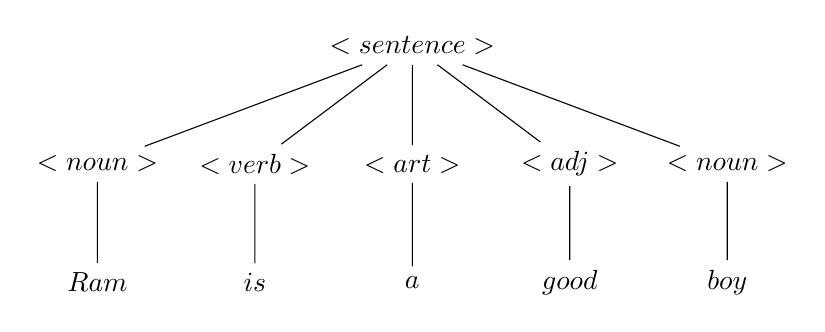
\begin{tikzpicture}[sibling distance=2cm]
\node {$<sentence>$}
child {node {$<noun>$}
	child {node {$Ram$}}
}
child {node {$<verb>$}
	child {node {$is$}}
}
child {node {$<art>$}
	child {node {$a$}}
}
child {node {$<adj>$}
	child {node {$good$}}
}
child {node {$<noun>$}
	child {node {$boy$}}
};
\end{tikzpicture}





\vspace{50pt}






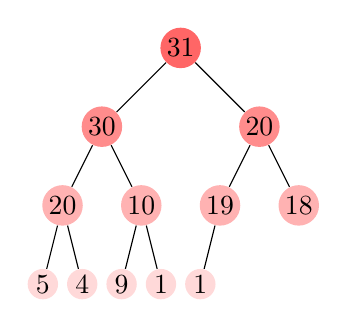
\begin{tikzpicture}[level distance=10mm]
\tikzstyle{every node}=[fill=red!60,circle,inner sep=1pt]
\tikzstyle{level 1}=[sibling distance=20mm,
set style={{every node}+=[fill=red!45]}]
\tikzstyle{level 2}=[sibling distance=10mm,
set style={{every node}+=[fill=red!30]}]
\tikzstyle{level 3}=[sibling distance=5mm,
set style={{every node}+=[fill=red!15]}]
\node {31}
child {node {30}
	child {node {20}
		child {node {5}}
		child {node {4}}
	}
	child {node {10}
		child {node {9}}
		child {node {1}}
	}
}
child {node {20}
	child {node {19}
		child {node {1}}
		child[fill=none] {edge from parent[draw=none]}
	}
	child {node {18}}
};
\end{tikzpicture}




\vspace{50pt}



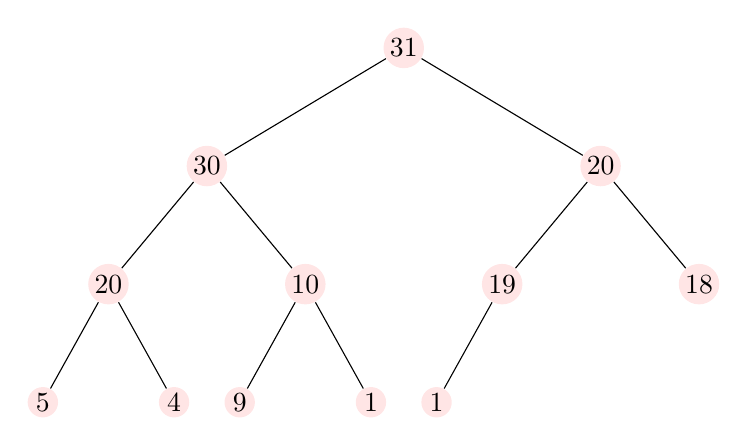
\begin{tikzpicture}[level/.style={sibling distance = 5cm/#1,
  level distance = 1.5cm}]
\tikzstyle{every node}=[fill=red!10,circle,inner sep=1pt]
%\tikzstyle{level 1}=[sibling distance=20mm,set style={{every node}+=[fill=red!45]}]
%\tikzstyle{level 2}=[sibling distance=10mm,set style={{every node}+=[fill=red!30]}]
%\tikzstyle{level 3}=[sibling distance=5mm,set style={{every node}+=[fill=red!15]}]
\node {31}
child {node {30}
	child {node {20}
		child {node {5}}
		child {node {4}}
	}
	child {node {10}
		child {node {9}}
		child {node {1}}
	}
}
child {node {20}
	child {node {19}
		child {node {1}}
		child[fill=none] {edge from parent[draw=none]}
	}
	child {node {18}}
};
\end{tikzpicture}





\vspace{50pt}







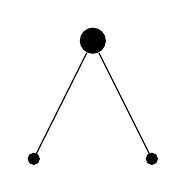
\begin{tikzpicture}
\node[circle,fill=black,minimum width=8pt] {}
child {[fill] circle (2pt)}
child {[fill] circle (2pt)};
\end{tikzpicture}



\vspace{50pt}





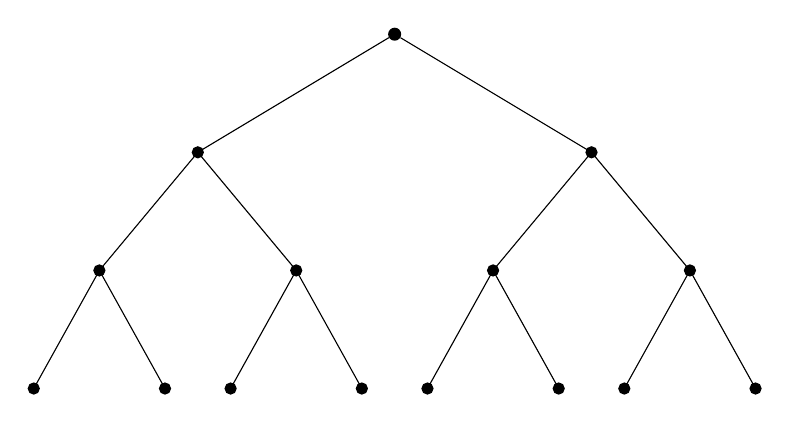
\begin{tikzpicture}[level/.style={sibling distance = 5cm/#1,
  level distance = 1.5cm}]
\node[circle,fill=black,scale=0.5] {}
child { [fill] circle (2pt)
	child { [fill] circle (2pt)
		child { [fill] circle (2pt)}
		child { [fill] circle (2pt)}
	}
	child { [fill] circle (2pt)
		child { [fill] circle (2pt)}
		child { [fill] circle (2pt)}
	}
}
child {[fill] circle (2pt)
	child { [fill] circle (2pt)
		child { [fill] circle (2pt)}
		child { [fill] circle (2pt)}
	}
	child { [fill] circle (2pt)
		child { [fill] circle (2pt)}
		child { [fill] circle (2pt)}
	}
};
\end{tikzpicture}




\vspace{50pt}





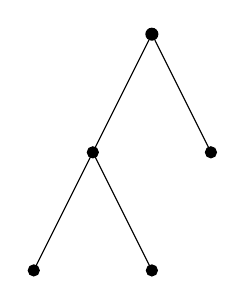
\begin{tikzpicture}
\node[circle,fill=black,scale=0.5] {}
child { [fill] circle (2pt)
	child { [fill] circle (2pt)}
	child { [fill] circle (2pt)}
}
child {[fill] circle (2pt)};
\end{tikzpicture}





\vspace{50pt}






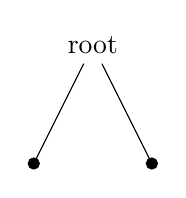
\begin{tikzpicture}
\node {root}
child {[fill] circle (2pt)}
child {[fill] circle (2pt)};
\end{tikzpicture}





\vspace{50pt}




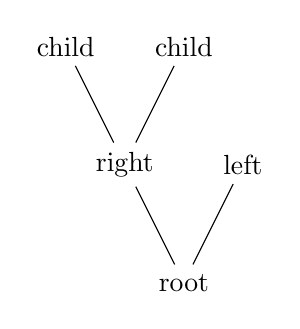
\begin{tikzpicture}
\node {root} [grow=up]
child {node {left}}
child {node {right}
child {node {child}}
child {node {child}}
};
\end{tikzpicture}




\vspace{50pt}





\begin{tikzpicture}
\node {root} [grow=right]
	child {node {left}
	}
	child {node {right}
		child[missing] {node {child}}
		child {node {child}
			child {node {child}}
			child[missing] {node {child}}
		}
	};
\end{tikzpicture}





\vspace{50pt}







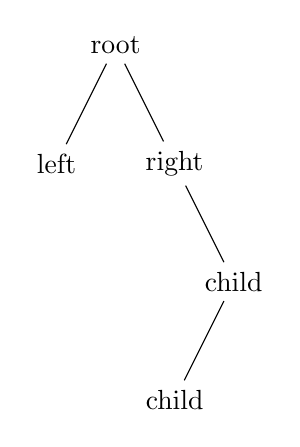
\begin{tikzpicture}
\node {root}
	child {node {left}
	}
	child {node {right}
		child[missing] {node {child}}
		child {node {child}
			child {node {child}}
			child[missing] {node {child}}
		}
	};
\end{tikzpicture}







\vspace{50pt}









\begin{center}
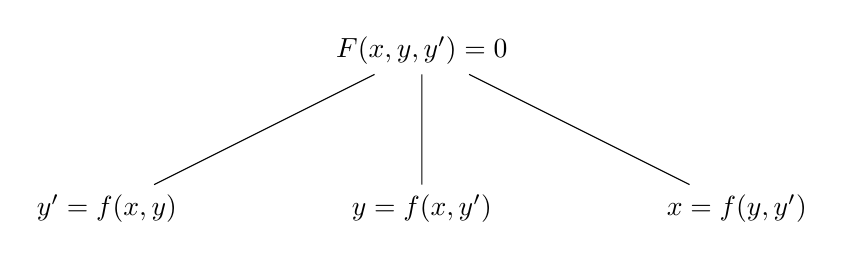
\begin{tikzpicture}[node distance = 1cm,level distance = 2cm,sibling distance = 4cm]
\node {$F(x,y,y') = 0$}
child {node {$y' = f(x,y)$}}
child {node {$y = f(x,y')$}}
child {node {$x = f(y,y')$}
};
\end{tikzpicture}
\end{center}






\vspace{50pt}






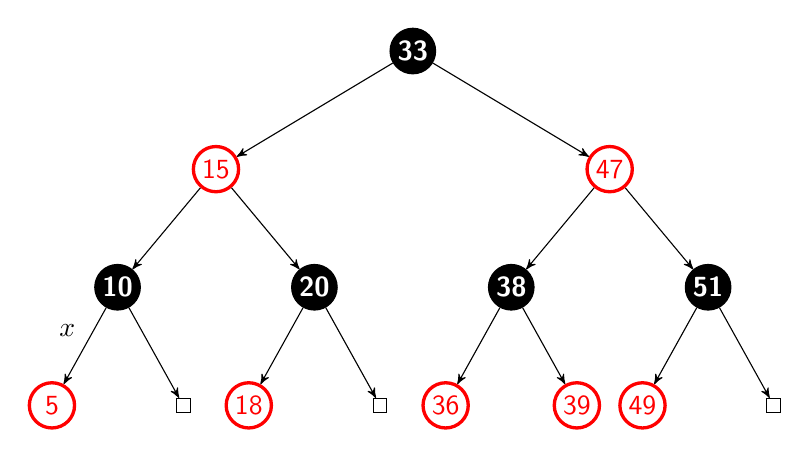
\begin{tikzpicture}[->,>=stealth',level/.style={sibling distance = 5cm/#1,
  level distance = 1.5cm}] 
  \tikzset{
  treenode/.style = {align=center, inner sep=0pt, text centered,
    font=\sffamily},
  arn_n/.style = {treenode, circle, white, font=\sffamily\bfseries, draw=black,
    fill=black, text width=1.5em},% arbre rouge noir, noeud noir
  arn_r/.style = {treenode, circle, red, draw=red, 
    text width=1.5em, very thick},% arbre rouge noir, noeud rouge
  arn_x/.style = {treenode, rectangle, draw=black,
    minimum width=0.5em, minimum height=0.5em}% arbre rouge noir, nil
}


\node [arn_n] {33}
    child{ node [arn_r] {15} 
            child{ node [arn_n] {10} 
            	child{ node [arn_r] {5} edge from parent node[above left]
                         {$x$}} %for a named pointer
							child{ node [arn_x] {}}
            }
            child{ node [arn_n] {20}
							child{ node [arn_r] {18}}
							child{ node [arn_x] {}}
            }                            
    }
    child{ node [arn_r] {47}
            child{ node [arn_n] {38} 
							child{ node [arn_r] {36}}
							child{ node [arn_r] {39}}
            }
            child{ node [arn_n] {51}
							child{ node [arn_r] {49}}
							child{ node [arn_x] {}}
            }
		}
; 
\end{tikzpicture}






\vspace{50pt}





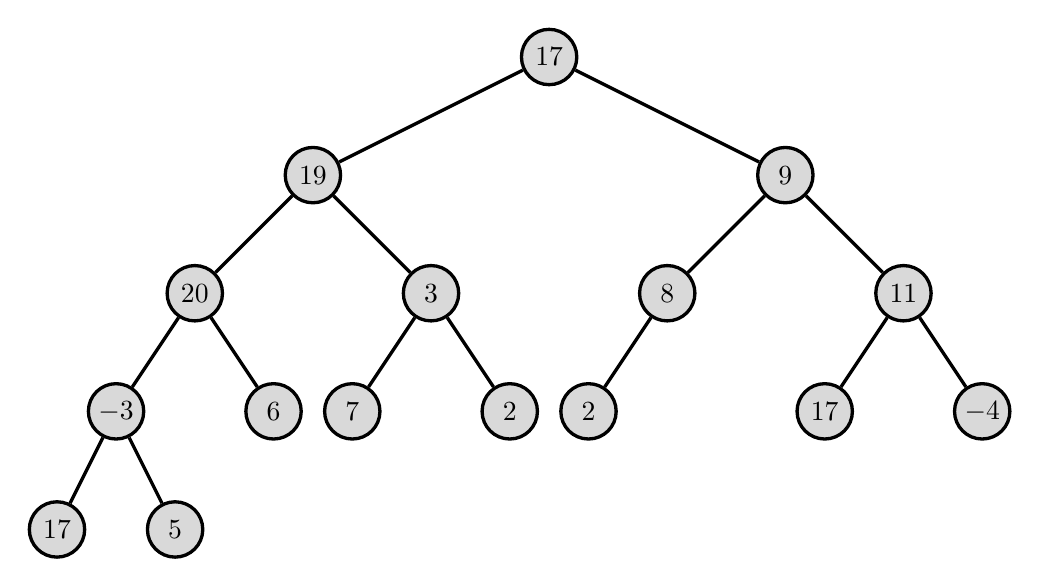
\begin{tikzpicture}[very thick,level/.style={sibling distance=60mm/#1}]
\tikzstyle{vertex}=[draw,fill=black!15,circle,minimum size=20pt,inner sep=1pt]
\node [vertex] (r){$17$}
  child {
	    node [vertex] (a) {$19$}
	    child {
		      node [vertex] {$20$}
		      child {
			        node [vertex] {$-3$}
			        child {node [vertex] {$17$}}
			        child {node [vertex] {$5$}}
		      }
		      child {node [vertex] {$6$}}
	    }
	    child {
		      node [vertex] {$3$}
		      child {node [vertex] {$7$}}
		      child {node [vertex] {$2$}}
	    }
  }
  child {
	    node [vertex] {$9$}
	    child {
		      node [vertex] {$8$}
		      child {node [vertex] {$2$}}
		      child [missing] {} 
	    }
	    child {
		      node [vertex] {$11$}
		      child {node [vertex] {$17$}}
		      child {node [vertex] {$-4$}}
	    }
  };
\end{tikzpicture}







\vspace{50pt}






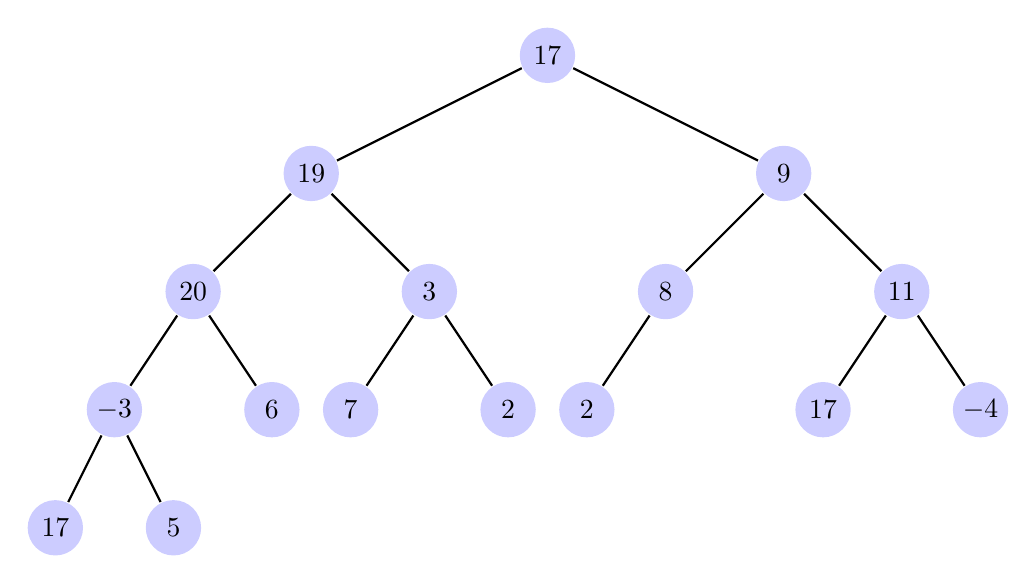
\begin{tikzpicture}[thick,level/.style={sibling distance=60mm/#1}]
\tikzstyle{vertex}=[circle,fill=blue!20,minimum size=20pt,inner sep=1pt]
\node [vertex] (r){$17$}
  child {
	    node [vertex] (a) {$19$}
	    child {
		      node [vertex] {$20$}
		      child {
			        node [vertex] {$-3$}
			        child {node [vertex] {$17$}}
			        child {node [vertex] {$5$}}
		      }
		      child {node [vertex] {$6$}}
	    }
	    child {
		      node [vertex] {$3$}
		      child {node [vertex] {$7$}}
		      child {node [vertex] {$2$}}
	    }
  }
  child {
	    node [vertex] {$9$}
	    child {
		      node [vertex] {$8$}
		      child {node [vertex] {$2$}}
		      child [missing] {} 
	    }
	    child {
		      node [vertex] {$11$}
		      child {node [vertex] {$17$}}
		      child {node [vertex] {$-4$}}
	    }
  };
\end{tikzpicture}




\vspace{50pt}





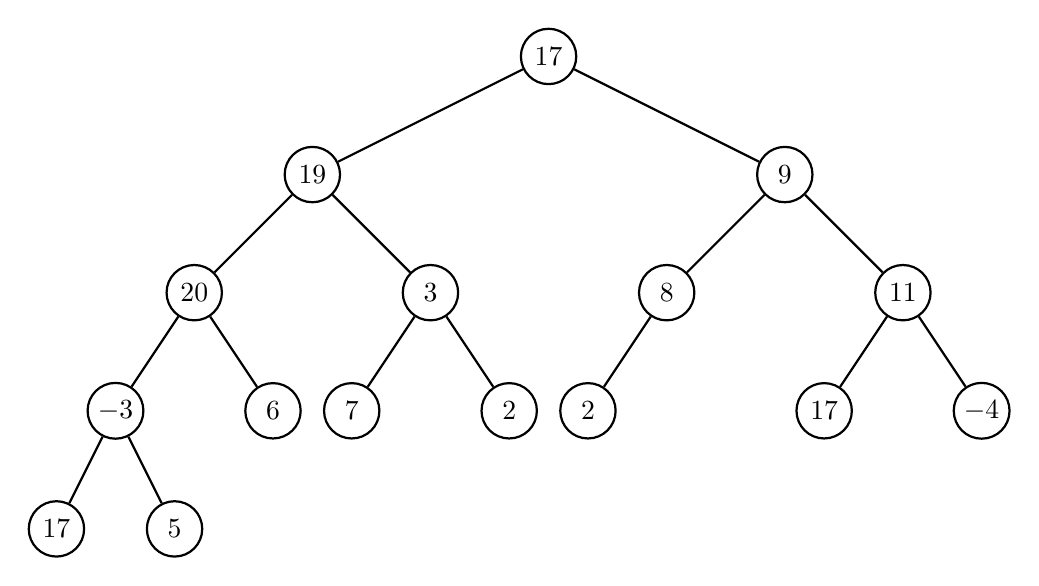
\begin{tikzpicture}[thick,level/.style={sibling distance=60mm/#1}]
\tikzstyle{vertex}=[draw,circle,fill=white,minimum size=20pt,inner sep=2pt]
\node [vertex] (r){$17$}
  child {
	    node [vertex] (a) {$19$}
	    child {
		      node [vertex] {$20$}
		      child {
			        node [vertex] {$-3$}
			        child {node [vertex] {$17$}}
			        child {node [vertex] {$5$}}
		      }
		      child {node [vertex] {$6$}}
	    }
	    child {
		      node [vertex] {$3$}
		      child {node [vertex] {$7$}}
		      child {node [vertex] {$2$}}
	    }
  }
  child {
	    node [vertex] {$9$}
	    child {
		      node [vertex] {$8$}
		      child {node [vertex] {$2$}}
		      child [missing] {} 
	    }
	    child {
		      node [vertex] {$11$}
		      child {node [vertex] {$17$}}
		      child {node [vertex] {$-4$}}
	    }
  };
\end{tikzpicture}




\vspace{50pt}






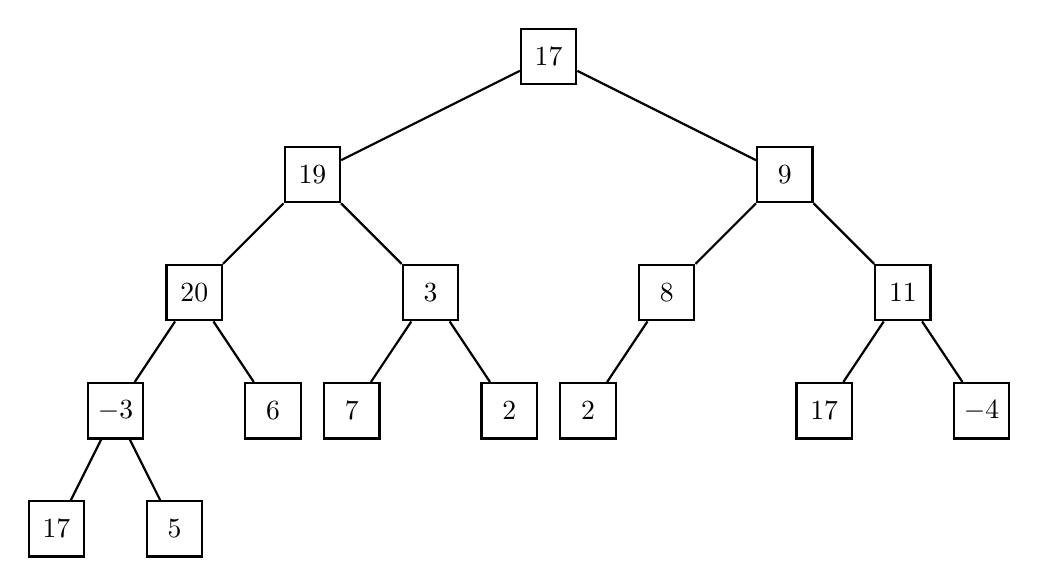
\begin{tikzpicture}[thick,level/.style={sibling distance=60mm/#1}]
\tikzstyle{vertex}=[draw,rectangle,fill=white,minimum size=20pt,inner sep=2pt]
\node [vertex] (r){$17$}
  child {
	    node [vertex] (a) {$19$}
	    child {
		      node [vertex] {$20$}
		      child {
			        node [vertex] {$-3$}
			        child {node [vertex] {$17$}}
			        child {node [vertex] {$5$}}
		      }
		      child {node [vertex] {$6$}}
	    }
	    child {
		      node [vertex] {$3$}
		      child {node [vertex] {$7$}}
		      child {node [vertex] {$2$}}
	    }
  }
  child {
	    node [vertex] {$9$}
	    child {
		      node [vertex] {$8$}
		      child {node [vertex] {$2$}}
		      child [missing] {} 
	    }
	    child {
		      node [vertex] {$11$}
		      child {node [vertex] {$17$}}
		      child {node [vertex] {$-4$}}
	    }
  };
\end{tikzpicture}





\vspace{50pt}






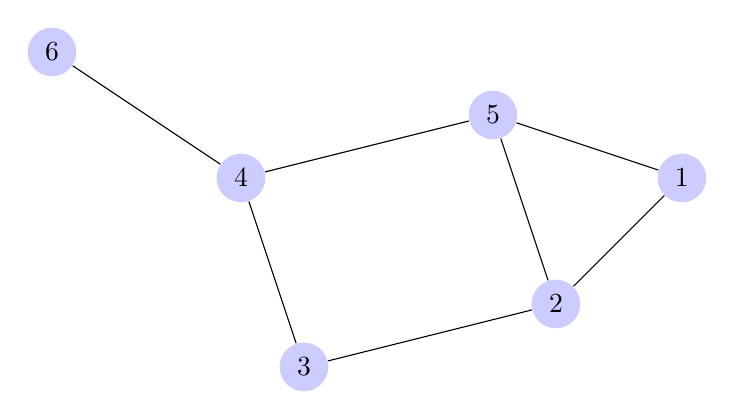
\begin{tikzpicture}
  [scale=.8,auto=left,every node/.style={circle,fill=blue!20}]
  \node (n6) at (1,10) {6};
  \node (n4) at (4,8)  {4};
  \node (n5) at (8,9)  {5};
  \node (n1) at (11,8) {1};
  \node (n2) at (9,6)  {2};
  \node (n3) at (5,5)  {3};

  \foreach \from/\to in {n6/n4, n4/n5, n5/n1, n1/n2, n2/n5, n2/n3, n3/n4}
    \draw (\from) -- (\to);
\end{tikzpicture}





\vspace{50pt}





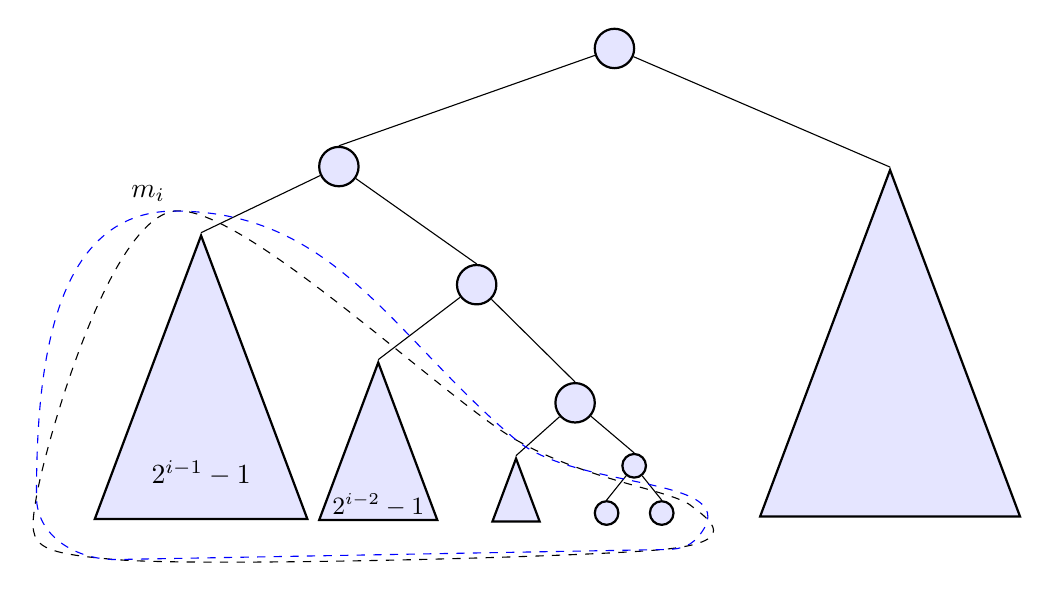
\begin{tikzpicture}[
  inner/.style={fill = light blue,circle,draw,thick,minimum width=5mm,inner sep=0},
  small inner/.style={inner,minimum width = 3mm},
  triangle/.style={fill = light blue,isosceles triangle,draw=,thick,shape border rotate=90,isosceles triangle stretches=true, minimum height=20mm,minimum width=15mm,inner sep=0,yshift={-10mm}},
  small triangle/.style={triangle, minimum height = 8mm, minimum width = 6mm },
  large triangle/.style={triangle,minimum width = 27mm,minimum height=36mm,yshift={-11mm}},
  very large triangle/.style={triangle,minimum width = 33mm,minimum height=44mm,yshift={-11mm}},
  level 1/.style={sibling distance=70mm},
  level 2/.style={sibling distance=35mm},
  level 3/.style={sibling distance=25mm},
  level 4/.style={sibling distance=25mm},
  level 4/.style={sibling distance=15mm},
  level 5/.style={sibling distance=7mm},
]
  \colorlet{light blue}{blue!10}
  \node[inner] {}
     [child anchor=north]
    child {node[inner] {}
        child {node[large triangle,yshift={-3mm}] (a) {$2^{i-1}-1$}}
        child {node[inner,yshift={0mm}] {}
            child{node[triangle,font=\small,yshift={-3mm}] (b) {$2^{i-2}-1$}}
            child{node[inner,yshift={0mm}] {}
                child{node[small triangle,font=\fontsize{6}{3},yshift={12mm}] (c) {}}
                child{node[small inner,yshift={7mm}]{}
                    child{node[small inner,yshift={9mm}] (d) {}}
                    child{node[small inner,yshift={9mm}] (e) {}}
                }
            }
        }
    }
    child {node[very large triangle ,yshift={-12mm}] {}};

\coordinate (A) at ([yshift=2.5cm,xshift=.5cm]a.north west);
\coordinate (B) at ([yshift=.2cm]c.north);
\coordinate (C) at ([xshift=.2cm,yshift=.1cm]e.east);
\coordinate (D) at ([xshift=.3cm,yshift=-.3cm]e.east);
\coordinate (E) at ([yshift=-.3cm]e.south);
\coordinate (F) at ([xshift=-.5cm,yshift=-.5cm]a.south west);
\coordinate (G) at ([xshift=-1.5cm,yshift=.3cm]a.south west);

\draw[dashed] plot[smooth cycle] coordinates {(A) (B) (C) (E) (F) (G)};

\draw [dashed,blue] (A) to[out=0,in=140]
      (B) to[out=320,in=50]
      (D) to[out=230,in=0] 
      (E) to
      (F) to[out=180,in=270]
      (G) to[out=90,in=180] (A);

\node at (A) [above  left] {\( m_i \)};
\end{tikzpicture}








\vspace{50pt}











\end{document}